%------------------------------------------------------------------------------
% Template file for the submission of papers to IUCr journals in LaTeX2e
% using the iucr document class
% Copyright 1999-2012 International Union of Crystallography
% Version 1.5 (7 March 2012)
%------------------------------------------------------------------------------

\documentclass[pdf]{iucr}
%\documentclass[preprint]{iucr}

\usepackage{bbold}
\usepackage{mathtools}
\usepackage{refstyle}
\usepackage{nomencl}
\usepackage[version=3]{mhchem}
\newref{eqn}{%
name={eqn~},
names={eqns~},
Name={Eqn~},
Names={Eqns~},
rngtxt={\ to~},
lsttxt={\ and~},
refcmd=(\ref{#1})
}
\newref{fig}{%
name={fig~},
names={figs~},
Name={Fig~},
Names={Figs~},
rngtxt={\ to~},
lsttxt={\ and~},
refcmd=(\ref{#1})
}
\newref{sec}{%
name={section~},
names={sections~},
Name={Section~},
Names={Sections~},
rngtxt={\ to~},
lsttxt={\ and~},
refcmd=\ref{#1}
}
\newref{appendix}{%
name={appendix~},
names={appendices~},
Name={Appendix~},
Names={Appendices~},
rngtxt={\ to~},
lsttxt={\ and~},
refcmd=\ref{#1}
}

\usepackage{tikz}
\usetikzlibrary{arrows,fit}

%%%%%%%%%%%%%%%%%%%%%%%%%%%%%%%%%%%%%% various notations %%%%%%%%%%%%%%%%%%%%%%%%%%%%%%%%%%%%%%%%%%%%

% programming
\newcommand{\code}[1]{\texttt{#1}}
\newcommand{\cpp}{C++}

% mathematical notations: convenience and centralised look
\newcommand{\mat}[1]{#1}
\newcommand{\re}{\operatorname{Re}}
\newcommand{\im}{\operatorname{Im}}
\newcommand{\identity}{\mathbb{1}}
\newcommand{\mean}[1]{\left\langle #1 \right\rangle}
\newcommand{\modulus}[1]{\left| #1 \right|}
\newcommand{\norm}[1]{\left\| #1 \right\|}
\newcommand{\sym}[2]{\left( #1\,\vert\, #2 \right)}
\newcommand{\inversion}{ \sym{\bar{1}}{t_{\bar{1}}} }
\newcommand{\cov}[2]{\mathrm{Cov}\left(#1,#2\right)}
\newcommand{\var}[1]{\mathrm{Var}\left(#1\right)}
\newcommand{\fourier}[1]{\mathrm{FFT}\left[#1\right]}
\newcommand{\kernel}{\operatorname{Ker}}
\newcommand{\image}{\operatorname{Im}}
\newcommand{\dimension}{\operatorname{dim}}
\newcommand{\tr}{\operatorname{Tr}}
\DeclareMathOperator{\dotprod}{\cdot}
\DeclareMathOperator{\crossprod}{\times}

\newcommand{\braket}[2]{\left\langle #1 \vphantom{#2} \right| \left. \vphantom{#1} #2 \right\rangle}
\newcommand{\argmax}{\operatornamewithlimits{argmax}}
\newcommand{\argmin}{\operatornamewithlimits{argmin}}
\newcommand{\partialder}[2]{\frac{\partial #1}{\partial #2}}
\newcommand{\partialderxx}[2]{\frac{\partial^2 #1}{\partial #2^2}}
\newcommand{\partialderxy}[3]{\frac{\partial^2 #1}{\partial #2 \partial #3}}
\newcommand{\grad}[2][]{%
        \ifthenelse{ \equal{#1}{} } { \nabla #2 }
                                              { \nabla_{#1} {#2} }
}
% crystallography
\newcommand{\uiso}{u_{\text{iso}}}

%%%%%%%%%%%%%%%%%%%%%%%%%%%%%%%%%%%%%%%%%%%%%%%%%%%%%%%%%%%%%%%%%%%%%%%%%%%%%%%%%%%%%%%%%%%%%%%%%%%%%%


\journalcode{A}           % Indicate the journal to which submitted
                                  %   A - Acta Crystallographica Section A
                                  %   B - Acta Crystallographica Section B
                                  %   C - Acta Crystallographica Section C
                                  %   D - Acta Crystallographica Section D
                                  %   E - Acta Crystallographica Section E
                                  %   F - Acta Crystallographica Section F
                                  %   J - Journal of Applied Crystallography
                                  %   S - Journal of Synchrotron Radiation

\begin{document}

\newcommand{\olexrefine}{Olex2.refine}

\addtolength{\parskip}{0ex plus 0.5ex minus 0.5ex}

\title{The Anatomy of a Comprehensive Constrained, Restrained, Refinement Program for the Modern Computing Environment -- Olex2 Dissected}
\shorttitle{\olexrefine}  % Abbreviated title for use in running heads

     % Authors' names and addresses. Use \cauthor for the main (contact) author.
     % Use \author for all other authors. Use \aff for authors' affiliations.
     % Use lower-case letters in square brackets to link authors to their
     % affiliations; if there is only one affiliation address, remove the [a].

\newcommand{\brukerfr}{Bruker AXS-SAS, 4 All\'ee Lorentz, 77447 Marne-la-Vall\'ee cedex 2, \country{France}}
\newcommand{\durhamchem}{Department of Chemistry, Durham University, South Road, Durham, DH1~3LE, \country{UK}}
\newcommand{\olexsys}{OlexSys Ltd, \durhamchem}
\newcommand{\cci}{CCI, Lawrence Berkeley Laboratory, 1 Cyclotron Road, BLDG 64R0121, Berkeley, CA 94720-8235, \country{USA}}
\newcommand{\diamondlight}{Diamond Light Source Ltd, Diamond House, Harwell Oxford, Didcot, Oxfordshire, OX11 0DE, \country{UK}}

\cauthor[\dagger]{Luc J.}{Bourhis}{luc\_j\_bourhis@mac.com}{}
\author[\ddagger]{Oleg V.}{Dolomanov}
\author[\S]{Richard J.}{Gildea}
\author[]{Judith A. K.}{Howard}
\author[\ddagger]{Horst}{Puschmann}

\aff[]{\durhamchem}
\aff[\dagger]{\brukerfr}
\aff[\ddagger]{\olexsys}
\aff[\S]{\diamondlight}


\shortauthor{Bourhis, Dolomanov, Gildea, Howard and Puschmann} % abbreviated author list for use in running heads

\keyword{small molecules}\keyword{refinement}\keyword{constraints}\keyword{restraints}\keyword{least-squares}

\newcommand{\latinit}[1]{\textit{#1}}

\maketitle

\newcommand{\ourEPSRCgrant}{EPSRC grant ``Age Concern: Crystallographic Software for the Future" (EP/C536274/1)}

\begin{synopsis}
Supply a synopsis of the paper for inclusion in the Table of Contents.
\end{synopsis}

\begin{abstract}
This paper describes the mathematical basis for \olexrefine, the new refinement engine which is integrated within the Olex2 program. We provide precise and clear equations for every computation performed by this engine, including structure factors and their derivatives, constraints, restraints and twinning, as well as a general overview of the different components of the engine and their relations to each others.
\end{abstract}

\section{Introduction}
\label{sec:introduction}
  
During the last four decades, small molecule crystallographers have used a myriad of stand-alone routines and various comprehensive software packages, most notably those written by George Sheldrick \cite{Sheldrick:2008aa,Sheldrick:1997aa} and that designed by Bob Carruthers and John Rollett, then maintained and enhanced by David Watkin \cite{Betteridge:2003ab}. These latter two packages have dominated the citations in all publications containing crystal structure analyses for many years now.

Therefore it might be claimed that the analysis of single crystal X-ray (and neutron) diffraction data has reached a certain level of maturity and that there is no need for further program development. Nonetheless there is still considerable activity in this area in various groups around the world and there has been a new release, SHELX 2013, from Sheldrick  recently. A retro-fit of new ideas to these older programs is not always possible, except perhaps by the authors themselves. 

\begin{figure}
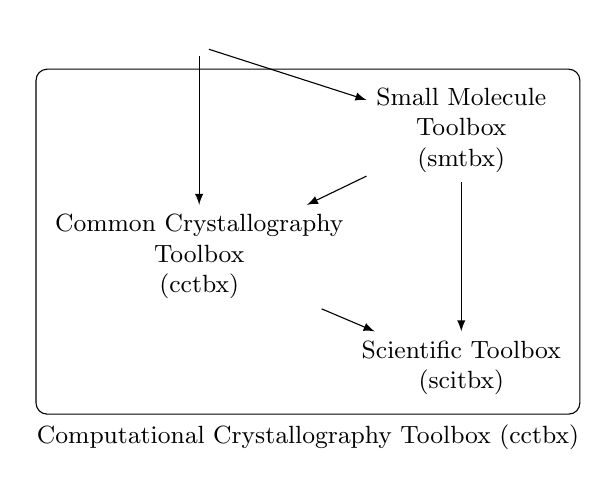
\begin{tikzpicture}[auto, dependency/.style=draw,-latex, border/.style=draw,rounded corners]
  \tikzstyle{every node}=[font=\small]
  \matrix[row sep=0.3cm, column sep=0]
  {
    \node (olex2) {\olexrefine}; & \\
    & \node[align=center] (smtbx) {Small Molecule \\ Toolbox \\ (smtbx)}; \\
    \node[align=center] (cctbx) {Common Crystallography \\ Toolbox \\ (cctbx)}; & \\
    & \node[align=center] (scitbx) {Scientific Toolbox \\ (scitbx)}; \\
  };
  \begin{scope}[every path/.style=dependency]
  \path (olex2) -- (smtbx);
  \path (olex2) -- (cctbx);
  \path (smtbx) -- (cctbx);
  \path (smtbx) -- (scitbx);
  \path (cctbx) -- (scitbx);
  \end{scope}
  \node[border, fit={(cctbx.west) (smtbx.north east) (scitbx.south east)}, draw,
        label=below:Computational Crystallography Toolbox (cctbx)] {};
\end{tikzpicture}
\caption{A high-level depiction of the software modules involved in \olexrefine: an arrow is drawn from each component pointing toward another component it uses.}
\label{fig:software:modules}
\end{figure}



When we first embarked on the project herein reported\footnote{\ourEPSRCgrant} we were clear about one point - namely that we wanted to create a new and flexible refinement engine, working in a collaborative environment and to be based on trusted and mature pre-existing code. This new refinement engine would be open source and therefore available for modification by others. Modern programming paradigms, unknown when the aforementioned packages were created in the 1960s, would form the basis of our development. It is hoped that such an architecture will allow extensions to the code without breaking the program or endangering the underlying functionality. It is this that we describe below in further detail and which now forms the underlying code for \olexrefine.\footnote{www.olex2.org}

We decided to base the computational core of \olexrefine\ on a pre-existing project, the Computational Crystallography Toolbox (cctbx), that provides the foundation for the macromolecular refinement facilities in the Phenix suite \cite{Adams:2010ys}. We made that choice because it provided the solid and versatile tools \cite{Grosse-Kunstleve:2003aa} that we needed to develop our project. The most important of them is a comprehensive and robust toolbox to handle crystal symmetries (sgtbx) that support every space group in any setting\footnote{Even rather unusual settings such as tripled cells can be built using the sgtbx}. Another key cctbx toolbox is the eltbx, which is concerned with scattering factor computations for any atom or ion and any wavelength that could be encountered in practice. The cctbx also featured many of the restraints we needed, in the module cctbx.restraints. 

For our project, we contributed to it a Small Molecule Toolbox (smtbx) which features, in particular, the constraint framework presented in detail in \secref{constraints} and \appendixref{constraints}, and the computation of structure factors presented in \appendixref{structurefactorlinearisation}. We also contributed several new restraints to cctbx.restraints which are discussed in \secref{restraints} and \appendixref{restraints}. Finally, both the cctbx and the smtbx use the Scientific Toolbox (scitbx) for arrays, matrices, special functions and other purely mathematical matters. We have contributed a new least-squares toolbox (lstbx) to the scitbx which provides flexible tools to deal with generic linear and non-linear problems, with or without an unknown overall scale factor. It implements the method based on normal equations presented in \appendixref{leastsquaresminimisation}.

The program Olex2 relies either on SHELX or on the smtbx to refine structures. If using the latter, Olex2 converts its internal model of a structure into the objects used by the smtbx and the cctbx to represent unit cell, reflections, crystal symmetry, constraints, restraints, \latinit{etc}. Once the smtbx has produced the desired results they are sent back to Olex2 which converts them to its own representations, so at to perform diverse post-processing and eventually display the results to the user of the program. \Figref{software:modules} summarises the dependencies between the various modules and programs that have just been described.  

\section{Least-Squares Refinement}
\newcommand{\data}{\text{data}}
\newcommand{\restraints}{\text{restraints}}

A small molecule structure refinement typically minimises the weighted least-squares function
\begin{equation}
\begin{split}
L = &\underbrace{\sum_h w_h \left( Y_{o,h} - K Y_{c,h} \right)^2}_{L_\data} \\
  &+ \underbrace{\sum_{\text{restraint } i} w_i \left( T_{o,i} - T_{c,i} \right)^2}_{L_\restraints}
\label{eqn:L:def}
\end{split}
\end{equation}
where $Y$ denotes either $F$ or $F^2$, and $K$ is an overall, unknown, scale factor that places the computed $Y_c$ on the same scale as the measured $Y_o$. The first sum over $h$ runs over a set of $m$ non-equivalent reflections that have been observed. Each observation is given an appropriate weight, $w_h$, based on the reliability of the measurement. These may be pure statistical weights, $w = 1/\sigma^2(Y_o)$, where $\sigma$ is the estimated standard deviation of the $Y_o$, though more complex weighting schemes are usually used. In the most general case, $w_h$ is a function of $Y_{o,h}$, $\sigma(Y_{o,h})$, $Y_{c,h}$ and $h$ itself, whereas the most common weighting schemes exhibit only a dependence on the first three.

These X-ray observations can be supplemented with the use of `observations of restraint', as suggested by \cite{Waser:1963aa}, where additional information, such as target values for bond lengths, angles \latinit{etc}. is included in the minimisation. This is the origin of the second term of the sum where $T_o$ is the target value for our restraint, and $T_c$ is the value of the target function calculated using the current model (see, for example \cite{Giacovazzo:2002aa,Watkin:2008aa}). This term $L_\restraints$ may of course be absent. Conversely, the data term could be absent in a refinement against geometrical terms only (\latinit{c.f.} the program DLS-76 \cite{Baerlocher:1978aa} for example).

In \eqnref{L:def}, the crystallographic parameters (i.e. atomic positions, atomic displacement parameters (ADPs), and chemical occupancy in routine refinements) that each component of $Y_c$ and $T_c$ depends upon will be collectively denoted as the vector $y=(y_1, \cdots, y_p)$ and we can therefore denote those dependencies with the compact notations $Y_c(y)$ and $T_c(y)$. The parameters that are actually refined may be a different set $x_1, \cdots, x_n$, collectively denoted as a vector $x$. We assume that the dependency of $y$ upon $x$ is known analytically. Since the scale factor $K$ is unknown, our problem is the minimisation of $L$ with respect to all of $K, x_1, \cdots, x_n$. We will  denotes that dependency as $L(y(x), K)$, or more tersely when we do not need to remember the crystallographic parameter vector $y$, as $L(x, K)$. These notations reflect the important fact that we treat the scale factor $K$ separately, as will be explained later.

For a small molecule structure with a high data to parameter ratio, such unconstrained minimisation as defined by the first term of \eqnref{L:def}, when $y \equiv x$ may well be sufficient. However, as the structure becomes larger, or the data to parameter ratio worsens, unconstrained minimisation may not be well-behaved, or result in some questionable parameter values. It has become customary to rely on the use of two techniques to solve such issues,
\begin{description}
\item[restraints:] by having a non-trivial second term in \eqnref{L:def} -- with the use of appropriate weighting of the restraints -- the minimisation is gently pushed towards giving a chemically sensible and hopefully correct structure;
\item[constraints:] by having a parameter vector $x$ shorter than $y$, therefore explicitly taking into account exact relationships between some of the parameters $y_i$.
\end{description}

Whether the refinement uses restraints or constraints or both, at each refinement cycle, we first find the value of $K$ that minimises $L(x, K)$ keeping the parameter vector $x$ fixed: we will denote it by $\tilde{K}(x)$, where we use a notation that is explicit in its dependency on the value of the refined parameters at the beginning of the cycle. We then search for the shift vector $s$ of the parameter vector $x$ that brings $L(x, \tilde{K}(x))$ closer to the minimum. It is solution of the so-called normal equations,
\begin{equation}
(B_\data + B_\restraints)s = -(g_\data + g_\restraints),
\label{eqn:generalnormalequations}
\end{equation}
where $B_\data$ and $B_\restraints$ are the so-called normal matrices associated with the two terms sharing the same labels in \eqnref{L:def} respectively and where the right hand side $g_\data$ and $g_\restraints$ are equivalently associated with those two terms (see the derivation of \eqnref{gaussnewtoneq} in \appendixref{leastsquaresminimisation}).

\Secref{constraints} deals with the computation of the derivatives with respect to the refined parameters $x_1, \cdots, x_n$ from the derivatives with respect to the crystallographic parameters $y_1, \cdots, y_p$. The computation of the latter derivatives is expounded in \appendixref{structurefactorlinearisation} along with the formulae for the complex structure factors $F_c$.

The computation of the normal equation terms $B_\data$ and $g_\data$ for the measured data is presented in details in \appendixref{leastsquaresminimisation} along with the procedure used to find the optimal value of $K$ whereas \secref{restraints} is devoted to the computation of $B_\restraints$ and $g_\restraints$.

\section{Constraints}
\label{sec:constraints}

\subsection{Synopsis}

The difference between restraints and constraints may be conceptualised mainly in two manners that we will first illustrate on a simple example: a geometrically constrained acetylenic hydrogen, \ce{X#C-H}. The position of the hydrogen must be such that the distance \ce{CH} is equal to some ideal bond length $d$ and such that the angle $\widehat{\ce{XCH}}$ is equal to $180^\circ$. Expressed in such an implicit manner, those restrictions could be used to construct restraints by adding to the function to minimise a term $w_1 (\ce{CH} - d)^2 + w_2 (\cos \widehat{\ce{XCH}} - 1)^2$. By doing so, the number of refined parameters would not be changed but the number of observations would increase by three. 

It is however traditional to do the opposite, by reducing the number of parameters by 3 and keeping the number of observations unchanged. This is achieved by using the implicit form of the constraints to express the position of \ce{H} as a function of the positions of the two carbon atoms. Denoting by $x$ the triplet of coordinates of the atoms,
\begin{equation}
x_\ce{H} = x_\ce{C} + d \frac{x_\ce{C} - x_\ce{X}}{\norm{x_\ce{C} - x_\ce{X}}},
\end{equation} 
where $\norm{.}$ denotes the Euclidean norm. By using this formula, the observable $Y_c$ of the fit (either $\modulus{F_c}^2$ or $\modulus{F_c}$) that used to depend on $x_\ce{C}$, $x_\ce{X}$ and $x_\ce{H}$ is replaced by a function $\tilde{Y}_c$ of $x_\ce{C}$ and $x_\ce{X}$ but not of $x_\ce{H}$. We will call this transformation a reparametrisation: $\tilde{Y}_c(x_\ce{C}, x_\ce{X}) = Y_c(x_\ce{C}, x_\ce{X}, x_\ce{H}(x_\ce{C}, x_\ce{X}))$ and we will say that $x_\ce{H}(x_\ce{C}, x_\ce{X})$ is a reparametrisation of $x_\ce{H}$, whose arguments are $x_\ce{C}$ and $x_\ce{X}$. The derivatives for the remaining variables are then obtained with the chain rule\footnote{For a column vector $x=\begin{pmatrix}x_1\\ x_2\\ x_3\end{pmatrix}$, $\partialder{F}{x}$ will always denote the row vector $\left(\partialder{F}{x_1}, \partialder{F}{x_2}, \partialder{F}{x_3}\right)$. Given another column vector $y=\begin{pmatrix}y_1\\ y_2\\ y_3\end{pmatrix}$, $\partialder{y}{x}$ will always denote the matrix $\left(\partialder{y_i}{x_j}\right)_{1 \le i,j \le 3}$ where $i$ (resp. $j$) indexes the rows (resp. the columns). The identity matrix will be denoted by $\identity$.},
\begin{align}
\partialder{\tilde{Y_c}}{x_\ce{C}} &= \partialder{Y_c}{x_\ce{C}} + \partialder{Y_c}{x_\ce{H}} \partialder{x_\ce{H}}{x_\ce{C}}, \\
\partialder{\tilde{Y_c}}{x_\ce{X}} &= \partialder{Y_c}{x_\ce{X}} + \partialder{Y_c}{x_\ce{H}} \partialder{x_\ce{H}}{x_\ce{X}}. \nonumber
\end{align}
It should be noted that it is customary to work within the ``riding" approximation,
\begin{align}
\partialder{x_\ce{H}}{x_\ce{X}} = 0,\ \partialder{x_\ce{H}}{x_\ce{C}} = \identity,
\end{align} 
which results in the much simplified chain rule
\begin{align}
\partialder{\tilde{Y}_c}{x_\ce{C}} &= \partialder{Y_c}{x_\ce{C}} + \partialder{Y}{x_\ce{H}}, \\
\partialder{\tilde{Y}_c}{x_\ce{X}} &= \partialder{Y_c}{x_\ce{X}}, \nonumber
\end{align}
implemented in all refinement programs, including Olex2.

It is not always the case that all three coordinates of an atom are removed from the refinement by constraints. For example, an atom in the plane of the mirror $z,y,x$ whose matrix reads
\begin{align}
M=\begin{bmatrix}
0 & 0 & 1\\
0 & 1 & 0\\
1 & 0 & 0
\end{bmatrix}
\end{align}
has its coordinates $x=(x_1, x_2, x_3)$ constrained by the relation $M x = x$, which can be reduced to $x_1 = x_3$ only. The corresponding reparametrisation may be written
\begin{align}
x_1 = u_1,\ x_2 = u_2,\ x_3 = u_1,
\label{eqn:specialposexamplereparam}
\end{align}
the observable $Y_c$ becoming now a function of the vector of newly introduced refinable parameters $u = (u_1, u_2)$. There is a general algorithm implemented in the cctbx that for any special position returns a matrix $Z$ so that the reparametrisation takes this form,\footnote{This algorithm first determines the space group symmetries that leaves the site invariant. The resulting system of linear equations, which read $M x = x$ in our example, is then reduced to a triangular form from which the matrix $Z$ and the vector $z$ are then readily obtained.}
\begin{align}
x = Z u + z
\end{align}
where $Z$ is a $3 \times 2$ or $3 \times 1$ matrix and $z$ is a 3-vector. This algorithm does not therefore try to determine which components of $u$, if any, are also components of $x$. This is why we have presented the reparametrisation for our example in this general form instead of keeping $x_1$ and $x_2$ as refinable parameters, which would sound more intuitive in the first place.
This matrix $Z$ is the matrix of constraints for the position of that atom. 

The anisotropic displacement tensor $U$ is subject to symmetry constraints as well. In our example, it must satisfy
\begin{align}
M U M^T = U,
\end{align}
where $M^T$ denotes the transpose of the matrix $M$. Any number of such matrix equations can always be rewritten as a system of equations whose most general form reads
\begin{align}
P &\begin{bmatrix}
U_{11}\\
U_{22}\\
U_{33}\\
U_{12}\\
U_{13}\\
U_{23}\\
\end{bmatrix} = 0.\label{eqn:exampleofadpconstraints}\\
\intertext{where P has 6 columns and $6n$ rows, where n is the number of symmetry elements involved in the special position. In our example} P &= \begin{bmatrix}
-1 & 0 & 1 & 0 & 0 & 0\\
0 & 0 & 0 & 0 & 0 & 0\\
1 & 0 & -1 & 0 & 0 & 0\\
0 & 0 & 0 & -1 & 0 & 1\\
0 & 0 & 0 & 0 & 0 & 0\\
0 & 0 & 0 & 1 & 0 & -1
\end{bmatrix}\\
\intertext{and \eqnref{exampleofadpconstraints} reduces to}
U_{11} &= U_{33}\text{ and } U_{12} = U_{23},\\
\intertext{leading to the constraint matrix}
\begin{bmatrix}
U_{11}\\
U_{22}\\
U_{33}\\
U_{12}\\
U_{13}\\
U_{23}\\
\end{bmatrix} &= \begin{bmatrix}
1 & 0 & 0 & 0\\
0 & 1 & 0 & 0\\
1 & 0 & 0 & 0\\
0 & 0 & 1 & 0\\
0 & 0 & 0 & 1\\
0 & 0 & 1 & 0
\end{bmatrix} \begin{bmatrix}
v_1\\
v_2\\
v_3\\
v_4
\end{bmatrix}
\end{align} 
Then one would refine $(v_1, v_2, v_3, v_4)$ instead of the $U_{ij}$.
The cctbx provides an algorithm that computes this matrix $P$ for any special positions, and then reduces it to triangular form in order to determine the constraint matrix for the ADP.

In other cases, a reparametrisation will make some crystallographic parameters disappear while introducing new refinable parameters. A typical example is that of a tetrahedral \ce{X-CH3} as the geometrical constraints leave one degree of freedom, a rotation about the axis \ce{X-C}. Thus the reparametrisation expresses the coordinates of the hydrogen atoms $H_0$, $H_1$ and $H_2$ as functions of the coordinates of the carbon atoms, and of an angle $\phi$ modelling that rotation,
\newcommand{\hydrogenphiarg}{\!\left(\phi\!+\!n \frac{2\pi}{3}\right)}
\begin{equation}
\begin{split}
x_\ce{H$_n$} = x_\ce{C} 
+ d \Biggl[ &\sin \alpha \left\{ \cos\hydrogenphiarg e_1 + \sin\hydrogenphiarg e_2 \right\}\\
- &\cos\alpha e_0
\Biggr],
\end{split}
\label{eqn:rotatingch3reparam}
\end{equation}
where $\alpha \approx 109.5^\circ$ and $(e_0, e_1, e_2)$ is an orthonormal basis of column vectors with $e_0$ in the direction of the bond \ce{X\bond{->}C}. The riding approximation in this case consists of neglecting the derivatives of those base vectors, leading to
\begin{align}
\partialder{\tilde{Y}_c}{x_\ce{C}} &= \partialder{Y_c}{x_\ce{C}} + \partialder{Y_c}{x_\ce{H}},\\
\partialder{\tilde{Y}_c}{x_\ce{X}} &= \partialder{Y_c}{x_\ce{X}}, \nonumber \\
\partialder{\tilde{Y}_c}{\phi} &= \partialder{Y_c}{x_\ce{H}} 
d \sin \alpha \left\{ -\sin\hydrogenphiarg e_1 + \cos\hydrogenphiarg e_2 \right\}. \nonumber
\end{align}
Thus a new derivative with respect to the new refinable parameter $\phi$ is introduced by this reparametrisation.

The last important concept is that of the chaining or composition of reparametrisations, that we will illustrate with a combination of the examples above\footnote{This example is not particularly common but it is a simple illustration of the concept we want to introduce.}. In the \ce{CH3} case, the atoms \ce{C} and \ce{X} could be on the special position studied in the next-to-last example. One type of disorder could be modelled by first applying the reparametrisation \eqnref[name=]{rotatingch3reparam} and then to reparametrise $x_\ce{C}$ and $x_\ce{X}$ using \eqnref{specialposexamplereparam}, introducing parameters $(u,v)$ for the former and $(u',v')$ for the latter. The derivatives would then be obtained by the chain rule, e.g.
\begin{equation}
\partialder{x_\ce{H0}}{u} = \partialder{x_\ce{H0}}{x_\ce{C}}\partialder{x_\ce{C}}{u} = 2
\end{equation}
in the riding approximation. This composition of reparametrisation may be represented as a graph: each parameter (some of them are triplets of coordinates, others are scalars), $x_\ce{H0}$, $x_\ce{H1}$, $x_\ce{H2}$, $x_\ce{C}$, $x_\ce{X}$, $\phi$, $u$, $v$, $u'$, and $v'$, constitutes a node of that graph, whereas edges are drawn from each node to its arguments, \latinit{i.e.} the nodes it depends upon, as shown on \figref{dependencegraphexample}. In this example, $x_\ce{C}$ has only one argument, $u$, whereas $x_\ce{H0}$ has three arguments, $x_\ce{C}$, $x_\ce{X}$ and $\phi$. The smtbx implements reparametrisations by explicitly building such a graph.

\begin{figure}
\begin{tikzpicture}[grow=left, every node/.style={circle,draw}, edge from parent/.style={-latex,draw}]
\node{$x_\ce{H0}$} child { node{$x_\ce{C}$}    child { node{$u$}  } }
                           child { node{$x_\ce{X}$} child { node{$u'$} } }
                           child { node{$\phi$} };
\end{tikzpicture}
\label{fig:dependencegraphexample}
\caption{Example of dependency graph for the chain of reparametrisation discussed in \secref{constraints}. Only the part for hydrogen atom $H_0$ is shown.}
\end{figure}


As models become more complex, e.g. hydrogen atoms riding on the atoms of a rigid body whose rotation centre is tied to an atom whose coordinates are refined, the reparametrisation graph becomes deeper. We decided not to put arbitrary limits on that graph. Indeed we could have made a closed list of reparametrisations and of reparametrisation combinations  that our framework would accept but instead we decided to write our code so that it could correctly handle the computation of parameter values and of partial derivatives for arbitrary reparametrisations, combined in arbitrary ways. This framework is therefore open as new type of reparametrisations can be added, without the need to change the basic infrastructure in any way, and without the risk of breaking existing reparametrisations. This has proven very useful to the authors as this enabled them to incrementally add the wealth of constraints now available, some of which are unique to \olexrefine, as discussed in \appendixref{constraints}. Furthermore, it enables third parties to develop their own constraints without the need for the involvement of the original authors beyond documenting how the reparametrisation framework works.

A crystallographic refinement may involve many such reparametrisations. By piecing them all together, we obtain one reparametrisation that expresses all refinable crystallographic parameters as a smaller vector of independent parameters that shall then be refined. Our framework safeguards that piecewise construction in several ways. First, at most one reparametrisation may be applied to any given parameter. An attempt to add a reparametrisation to a parameter that is already subject to one would be rejected by our framework as an error. Then if a cycle were found in the dependency graph, the framework would also reject the parametrisation. This would happen when at least one parameter, through a series of reparametrisation combinations, depends upon itself. Thus our framework safeguards against incorrect user inputs, and also against bugs in our own code that automatically builds constraints.

\subsection{Constraint matrix}

There are a wealth of algorithms designed to minimise least-squares but crystallographic software have only implemented a few of them. The two most popular methods have historically been the full-matrix\footnote{This method is also known as the Gauss-Newton algorithm.} (all small molecule programs, including Olex2, as explained in \appendixref{leastsquaresminimisation}), and Conjugate Gradient L.S. (CGLS) which SHELXL offers as an option along with full-matrix.  The macro-molecular community later introduced the Limited-memory Broyden-Fletcher-Goldfarb-Shanno method (LBFGS), \emph{phenix.refine} \cite{Afonine:2012aa}, and a sparse Gauss-Newton algorithm, REFMAC \cite[section 4 and references therein]{Murshudov:2011aa}. All methods mentioned above have in common the fact that they require only the computation of the value and the first-order derivatives of the calculated $F$ or $F^2$, that we have denoted as $Y_c$ in this paper. The fact that no higher-order derivatives are used greatly simplifies the implementation of constrained least-squares.

Indeed, after transforming every constraint on the model into a reparametrisation as explained and exemplified in the previous section and piecing all those reparametrisations together, we obtain a global reparametrisation of the vector of crystallographic parameters $y = (y_1, \cdots, y_p)$ as a function of the vector $x=(x_1, \cdots, x_n)$ of the parameters that are actually refined. It should be noted that any component $y_k$ of $y$ that is not reparametrised -- e.g. a coordinate of the pivot atom on which another atom rides, and of course any parameter that is not involved in any constraint --  is also a component $x_l$ of $x$, i.e. 
\begin{equation}
\partialder{y_k}{x_j} = \begin{cases} 
   1& \text{if $j=l$},\\
   0& \text{if $j \neq l$}.
   \end{cases}
\nonumber
\end{equation}

 From the known analytical expression of $Y_c(x)$, one computes the derivatives of $\partialder{Y_c}{y_i}$ (the reader is referred to \appendixref{structurefactorlinearisation} for a detailed presentation of those computations). The minimisation algorithm then only needs the derivatives of
\begin{align}
\tilde{Y}_c(x) &= Y_c(y(x)) \\
 \shortintertext{with respect to each $x_i$, which are easily obtained by a simple application of the chain rule,}
\partialder{\tilde{Y}_c}{x} &= \partialder{Y_c}{y} \partialder{y}{x}.
\label{eqn:chainrule}
\end{align}
The matrix $\partialder{y}{x}$ is known as the constraint matrix in crystallographic circles.\footnote{The earliest appearance of that concept in crystallographic litterature, though not by that name, brought to the attention of the authors is \cite{Larson:1980aa}} In standard mathematical nomenclatures, it is called the Jacobian of the transformation $x \mapsto y$ and we will therefore denote it $J$.

The computation of $J$ takes advantage of the fact that it is a very sparse matrix. This stems from the fact that any given crystallographic parameter $y_i$ depends on very few refined parameters $x_j$, as amply illustrated in the previous section. We take advantage of this property to drastically reduce the memory cost of $J$ and the cost of computing each of its non-zero coefficients. More precisely, both of these costs scale as the number of non-zero elements in $J$ instead of $O(n^2)$ if $J$ were treated as a dense matrix.

\section{Restrained Least-Squares Refinement}
\label{sec:restraints}

In this section we will give an overview of the computations involved in restrained refinement. The mathematical formulae for each restraint objective and their derivatives can be found in \appendixref{restraints}.

Since each restraint target $T_{c,i}$ only depends on a very small subset of the $y_j$ (e.g., in the case of a bond length, only the 6 coordinates of the two bonded atoms would play a role), the matrix of derivatives with respect to the crystallographic parameters
\begin{equation}
D_\restraints = \partialder{T_c}{y} = \left[\partialder{T_{c,i}}{y_j}\right]_{i,j},
\end{equation}
which is known as the design matrix for the restraints, is very sparse. We therefore use sparse matrix techniques to efficiently store and perform computations with $D$, by only storing non-zero elements, and never performing any multiplication that involves an element of $D$ known to be zero. We then introduce the matrix of derivatives with respect to the refined parameters,
\begin{equation}
\tilde{D}_\restraints = \partialder{T_c}{x} = D_\restraints \partialder{y}{x},
\label{eqn:constraints:applied:torestraints}
\end{equation}
which is computed by forming the product of $D$ and the constraint matrix. Thus the restraints are initially built up without any knowledge of the constraint matrix. This greatly simplifies their implementation and it simplifies their use in a refinement program that does not use constraints. This organisation of the computation does not incur any inefficiency as the product~\eqnref[name=]{constraints:applied:torestraints} is a cheap operation since both matrices are sparse, and it therefore scales as the number of non-zero elements, which is typically much smaller than the number of parameters $n$. 

The two terms in the normal equations~\eqnref[name=]{generalnormalequations} coming from the restraints then reads as the matrix product and matrix-vector product\footnote{$D^T$ denotes the transpose of $D$.},
\begin{align}
B_\restraints &= \tilde{D}_\restraints^T W \tilde{D}_\restraints\\
g_\restraints &= \tilde{D}_\restraints^T \Delta T,\\
\shortintertext{where $W$ is the diagonal matrix featuring the restraints weights, and where}
\Delta T_i &= T_{o,i} - T_{c,i}
\end{align}
is the residual for the $i$-th restraint. We take again advantage of the sparsity of $\tilde{D}_\restraints$ to efficiently implement those products.

It would be desirable to place the weights of the restraints on the same scale as the typical residual, such that a restraint will have a similar strength for the same weight in different structures. \cite{Rollett:1970ab} suggests the normalization factor
\begin{equation}
w_\restraints = \frac{1}{m-n} \sum_{h}{ w_h (Y_{o,h} - K Y_{c,h})^2}.
\label{eqn:giacovazzo_normalisation}
\end{equation}
This is better known as the square of the \emph{goodness of fit}, $\chi^2$. This normalising factor also allows the restraints to have greater influence when the fit of the model to the data is poor (and the goodness of fit is greater than unity), whilst their influence lessens as the fit improves \cite{Sheldrick:1997aa}.

\subsection{Implementation}

The choice of the minimisation algorithm has a significant impact on the organisation of the computation of restraints. Indeed, a generic minimiser such as the LBFGS minimiser used in \emph{phenix.refine} \cite{Afonine:2012aa} requires at each iteration only the function value $L$ and the derivatives $\partialder{L}{x}$. The derivatives $\partialder{L_\data}{x}$ and $\partialder{L_\restraints}{x}$ can be calculated separately before combining their sum to obtain $\partialder{L}{x}$. In contrast, for full-matrix least-squares we need the matrices of partial derivatives $\partialder{F_c}{x}$ and $\partialder{T_c}{x}$. Therefore, depending on the optimisation method used, we must be able to compute both $\partialder{L}{x}$ and $\partialder{T_c}{x}$ where, by the chain rule,
\begin{align}
\partialder{L_\restraints}{x} &= \partialder{L}{T_c} \partialder{T_c}{x} \nonumber\\
                             &= 2 w \left(T_o - T_c \right) \partialder{T_c}{x}.
\end{align}

The restraints framework was designed in such a way that it could be easily extended by adding further restraints. Each restraint must provide the array of partial derivatives of the restraint with respect to the crystallographic parameters (one row of the matrix $\partialder{T_c}{y}$), the restraint delta, $T_o - T_c$, and the weight, $w$, of the restraint.


\section{Twinning}
\label{sec:ls_twinning}

As all other refinement programs, we have adopted the model of twins proposed by \cite{Jameson:1982aa} and \cite{Pratt:1971aa}. The sample is modelled as $d$ domains, each sizeable enough a single crystal to give rise to observable Bragg peaks. If peaks from different domains fall very close in reciprocal space, the integration software analysing frames will be able to compute only the sum of the intensities of these superposed peaks. Data for the $r$-th reflection will therefore consist in an intensity $F_{o,r}^2$ and in a list of $s_r$ Miller indices $h_{r,i_1}, h_{r,i_2}, \cdots, h_{r,i_{s_r}}$ where $h_{r,i}$ is the triplet of Miller indices of the Bragg peak originating from diffraction by domain $i$. The model of the structure then predicts an intensity $I_{c,r}$ for $F_{o,r}^2$ that reads
\begin{align}
\label{eqn:twinnedintensity}
I_{c,r} &= \sum_{l=1}^{s_r} \alpha_{i_l} |F_c(h_{r,i_l})|^2\\
\shortintertext{where $\alpha_i$ is the fraction of the sample volume occupied by twin domain $i$. The least-squares to minimise are then, adapting \eqnref{L:def} for a twinned structure,}
L &= \sum_{r=1}^m w_r \left(F_{o,r}^2-K I_{c,r}\right)^2
\shortintertext{where the weight $w_r$ is usually}
w_r &= w(F_{o,r}^2, \sigma(F_{o,r}^2), I_{c,r})\\
\shortintertext{where $w$ would be the same function discussed in the context of \eqnref{L:def}. The minimisation of $L$ with respect to the model parameters embodied in $F_c$ and with respect to the $\alpha$'s is therefore subject to the constraint}
1 &= \sum_{i=1}^d \alpha_i.
\end{align}

There is a special case that is common and therefore important, where there are exactly $d$ superposed peaks for each reflection, i.e., $s_r=d$ for every $r$, and where there is a symmetry operator $R$, the twin law, that generates the Miller indices for each domain $i > 1$, as
\begin{align}
h_{r,i}=Rh_{r,i-1};
\end{align}
in this case, the input consists solely of a list of $F_o(h)^2$ (as for a untwinned refinement but with $h=h_{r,1}$) and of $R$. Such twins belong to the taxonomies pseudo-merohedral or merohedral. \olexrefine\ is able to refine a twinned structure input in this manner.

The general case would be handled by using a reflection file in the HKLF5 format by SHELXL users. Such a file is created by the integration software and this approach can deal with the most complex situations. By contrast, CRYSTALS always requires a list of twin laws.

\olexrefine\ can handle a more general case: when non-merohedral and merohedral twinning are simultaneously present. For example, one may have 4 domains 1, 2, 3 and 4. Domain 1 and 3 are related by a symmetry operator $R$, and so are domain 2 and 4, but the relative orientation of domain 1 and 2 does not correspond to any symmetry operator. Thus the measured frames exhibit 2 lattices of Bragg peaks, with some overlaps, and the integration software will then output a list of ($F_o^2$, $h_1$), ($F_o^2$, $h_2$) and ($F_o^2$, $h_1$, $h_2$). The refinement engine needs to expand this to a list of ($F_o^2$, $h_1$, $h_3=Rh_1$), ($F_o^2$, $h_2$, $h_4=Rh_2$), and ($F_o^2$, $h_1$, $h_2$, $h_3=Rh_1$, $h_4=Rh_2$). \olexrefine\ performs this task on the fly, while passing Miller triplets to the code computing structure factors and their derivatives.

The theory and phenomenology of twinning extends far beyond our exposition but from the narrow point of view of refinement, our presentation is sufficient, since, in this paper, we do not concern ourselves with the computation of the twin law or with the indexing of superposed lattices.


\section{Standard Uncertainties}
\label{sec:errors}

\subsection{Variance Matrix}
\label{sec:variance:matrix}

In this section, we will discuss the rigorous computation of standard uncertainties (s.u.) of and correlation between the parameters of a constrained model. As pointed out in \appendixref{leastsquaresminimisation} in the comment about \eqnref{gaussnewtonaslinearls}, the variance matrix for the refined parameters $x$ is
\begin{align}
\var{x} &= B^{-1}\\
\shortintertext{where}
B_{ij} &= \partialder{r}{x_i} \dotprod \partialder{r}{x_j}
\end{align}
is the normal matrix for the constrained least-squares minimisation. However, we are interested in the variance matrix $\var{y}$ for the crystallographic parameters of the model, not in $\var{x}$. For small variations, we have the linear relation
\begin{align}
\delta y &\approx J \delta x\\
\shortintertext{and therefore, using the well-known heuristic definition of the variance matrix of $y$ as the mean value of $\delta y \delta y^T$ in the linear approximation around the minimum implicitly assumed throughout crystallographic refinement,}
\var{y} &= J\, \var{x} J^T.
\label{eqn:constrained:variance:matrix}
\end{align} 

We would like to stress an important consequence of this formula: constrained parameters generally have non-zero standard uncertainties (s.u.). This is the case for example of the coordinates of riding atoms.\footnote{For most constraints, the s.u. of Hydrogen coordinates are equal to the s.u. of the atom they ride on but e.g. for a rotating \ce{-CH_3}, they differ because the s.u. of the azimuthal angle increases the s.u. of the Hydrogen coordinates that comes from riding only.} 

\subsection{Derived parameters}

We will now discuss the s.u. of derived parameters. Such a parameter is a function $f$ of a set of atomic parameters $p_i$ and its variance can be derived using the same heuristic as above in a linear approximation where $\delta f \approx \sum_i \partialder{f}{p_i} \delta p_i$ by computing $\var{f}$ as the mean of $(\delta f)^2$. This leads to
\begin{equation}
\sigma^2(f) = \sum_{i,j}{\left(\partialder{f}{p_i}\right) \left(\partialder{f}{p_j}\right) cov(p_i,p_j)}.
\label{eqn:sigma_f}
\end{equation}
An early occurence of this formula can be found in \cite{Sands:1966bh}.

As a result of this formula and of the consequence of \eqnref{constrained:variance:matrix} stated after it, any bond length, any bond angle and any dihedral angle involving a riding atom has a non-zero s.u. unless that geometrical quantity is fixed by the constraint. For example, in the case of \ce{(R1$,\,$ R2$,\,$ R3)-C-H}, for which the constraints does not fix the angles $\widehat{\ce{R$_i$CH}}$, those angles have a non-zero s.u. This correct behaviour unfortunately triggers many alerts when a structure refined with Olex2 is checked with PLATON. 

PLATON plays a very important role in detecting common flaws in the crystallographic workflow. However since PLATON does not have access either to the covariance matrix or the constraint matrix, it has to make guesses that results in estimation of esd's that may be out by up to a factor 2. This is the key problem we encounter with the way \olexrefine\ reports esd's. Specifically, most structure refined with \olexrefine\ fails checkCIF test PLAT732 (an alert C), for the reason explained in the documentation of this alert (in Note 2):\footnote{This note seems to be a recent addition and the authors would like to thank Ton Spek for this helpful consideration.} PLATON computes the s.u. of the said angle using the s.u. of the atomic coordinates as if they were independent parameters as it does not have access to the variance-covariance matrix that describes their correlations. In this case, those correlations are very significant since the position of H completely depends on the position of R1, R2 and R3. Hence the s.u. of this angle as reported by Olex2 differs from PLATON estimate. Thus all failures of test PLAT732 for angles or distances involving constrained Hydrogen atoms are spurious. As a result, if a referee were to require that all alerts C are to be addressed in a CIF submitted for publications in Acta Crystallographica, we advise authors to explain away PLAT732 for riding Hydrogen atoms by quoting note 2 in the documentation for that test. \olexrefine\ will actually automatically prepare the CIF file with such explanations.

\subsubsection{Incorporating s.u. of unit cell parameters}

Derived parameters such as bond lengths and angles are a function of both the least-squares atomic parameters and the unit cell parameters. As such, the s.u. of a derived parameter is likewise a function of both the atomic and unit cell parameters as well as their respective s.u. If the s.u. in atomic parameters are considered to be totally uncorrelated with the s.u. in the cell parameters (\emph{i.e.} their covariance is zero), then the s.u. in a derived parameter can be considered as comprising two independent sources of uncertainties:

\begin{equation}
\sigma^2(f) = \sigma^2_{cell}(f) + \sigma^2_{xyz}(f)
\label{eqn:sigma_d},
\end{equation}
where $\sigma_{xyz}(f)$ is the part coming from the uncertainties in the least square estimates of the positional parameters, and $\sigma_{cell}(f)$ comes from the uncertainties in the unit cell parameters,
\begin{equation}
\sigma^2_{cell}(f) = \sum_{i,j}{{\partialder{f}{i}\partialder{f}{j} cov\left(i,j\right)}}
\label{eqn:sigma_cell},
\end{equation}
where $i,j=\lbrace{a,b,c,\alpha,\beta,\gamma\rbrace}$.

This necessitates the calculation of the derivatives of the function with respect to the unit cell parameters. In order to do so, it is easier to calculate separately the derivatives of the function with respect to the elements of the metrical matrix, and also the derivatives of the metrical matrix with respect to the cell parameters, and then to use the chain rule

\begin{equation}
\partialder{f}{i} = \partialder{f}{g_{jk}}\partialder{g_{jk}}{i},\ i=a, b, c, \alpha, \beta, \gamma.
\label{eqn:df_dcell}
\end{equation}
Indeed $\partialder{f}{g_{jk}}$ must be evaluated for every function, whereas $\partialder{g_{jk}}{i}$ is constant for a given unit cell.

Now we consider the application of \eqnref{sigma_f} to determine the s.u. in the length of the vector $u$, in fractional coordinates. The length, $D$, of the  vector $u$ is given by
\begin{equation}
D = (u^T \mat{G} u)^\frac{1}{2}
\label{eqn:bond_length},
\end{equation}
where $\mat{G}$ is the metrical matrix.

The derivatives of the distance, $D$, with respect to the elements of the metrical matrix, $\mat{G}$, are given by

\begin{equation}
\partialder{D}{g_{ii}} = \frac{1}{2} \frac{u_i^2}{D}
\label{eqn:d_distance_d_gii}
\end{equation}
and (given the metrical matrix is symmetric)
\begin{equation}
\partialder{D}{g_{ij}} = \frac{u_i u_j}{D},\ \text{for all $i<j$}.
\label{eqn:d_distance_d_gij}
\end{equation}

Similarly, for the angle between two vectors in fractional coordinates, $u$ and $v$, where the angle is defined as
\begin{align}
\theta &= \arccos \frac{u^T\mat{G}v}{\norm{u^T\mat{G}u}\norm{v^T\mat{G}v}} \\
%\label{eqn:angle_frac}
\shortintertext{or}
\theta &= \arccos \frac{r_{A}\cdot r_{B}}{\norm{r_{A}}\norm{r_{B}}}
\label{eqn:angle_cart},
\end{align}
where $r_{A}$ and $r_{B}$ are the Cartesian equivalents of $u$ and $v$. The derivative of the angle, $\theta$, with respect to the elements of the metrical matrix, $\mat{G}$, is given by
\begin{equation}
\partialder{\theta}{g_{ii}} = \frac{1}{2 \sin\theta} \left(\frac{u_i^2 \cos{\theta}}{\norm{r_{A}}^2} - \frac{2 u_i v_i }{\norm{r_{A}}\norm{r_{B}}} +\frac{v_i^2 \cos{\theta}}{\norm{r_{B}}^2}\right)
\label{eqn:d_angle_d_gii}
\end{equation}
and
\begin{multline}
\partialder{\theta}{g_{ij}} = \frac{1}{\sin\theta} \left(\frac{u_i u_j \cos{\theta}}{\norm{r_{A}}^2} - \frac{u_i v_j + u_j v_i }{\norm{r_{A}}\norm{r_{B}}} +\frac{v_i v_j \cos{\theta}}{\norm{r_{B}}^2}\right),\\ \text{for all $i<j$}.
\label{eqn:d_angle_d_gij}
\end{multline}

\newcommand{\cell}{C}
The derivative of the metrical matrix with respect to the unit cell parameters, 
\begin{align}
\cell =& (a, b, c, \alpha, \beta, \gamma)\\
\shortintertext{needed in order to apply equation \eqnref{df_dcell}, are given below:}
\partialder{g_{11}}{\cell} =& \left(2 a,0,0,0,0,0\right) \\ \nonumber
\partialder{g_{22}}{\cell} =& \left(0,2 b,0,0,0,0\right) \\ \nonumber
\partialder{g_{33}}{\cell} =& \left(0,0,2 c,0,0,0\right) \\ \nonumber
\partialder{g_{12}}{\cell} =& \left(b \cos\gamma,a \cos\gamma,0,0,0,-a b \sin\gamma\right) \\ \nonumber
\partialder{g_{13}}{\cell} =& \left(c \cos\beta,0,a \cos\beta,0,-a c \sin\beta,0\right) \\ \nonumber
\partialder{g_{23}}{\cell} =& \left(0,c \cos\alpha,b \cos\alpha,-a c \sin\beta,0,0\right) \nonumber
\end{align}

\subsection{Symmetry}
The variance-covariance matrix that is obtained from the inversion of the least-squares normal matrix contains the variance and covariance of all the refined parameters. Frequently, it is necessary to compute functions that involve parameters that are related by some symmetry operator of the space group to the original parameters. \cite{Sands:1966bh} suggests that the symmetry should be applied to the variance-covariance matrix to obtain a new variance-covariance matrix for the symmetry generated atoms. Alternatively, and it is this method that is used here, the original variance-covariance matrix can be used if the derivatives in \eqnref{sigma_f} are mapped back to the original parameters.

Let the function $f$ depend on the Cartesian site $y_c$ that is generated by the symmetry operator $\mat{R}_c$ from the original Cartesian site $x_c$, \emph{i.e.}
\begin{align}
y_c &= \mat{R}_c x_c.\\
\shortintertext{Then the gradient with respect to the original site can be obtained by}
\partialder{f(y_c)}{x_c} &= \partialder{f(y_c)}{y_c} \mat{R}_c
\label{eqn:symmetry_derivative}.
\end{align}

The variance-covariance matrix that is used in this case should be the one that is transformed to Cartesian coordinates. The variance-covariance matrix for Cartesian coordinates can be obtained from that for fractional coordinates by the transformation

\begin{equation}
\mat{V}_{c} = \mat{\mathcal{O}} \mat{V}_{f} \mat{\mathcal{O}}^{T}.
\label{eqn:vcv_cart}
\end{equation}
where the transformation matrix $\mathcal{O}$ needed to transform the entire variance-covariance matrix in one operation would be block diagonal, with the $3 \times 3$ orthogonalisation matrix $O$ repeated at the appropriate positions along the diagonal. This transformation can be computed efficiently using sparse matrix techniques.

\section{Refinement results}

\olexrefine\ uses CIF \cite{Hall:1991aa} as its main output. The CIF contains information regarding the space group, the data indicators such as merging indices, the refinement indicators such as the R factors, goodness of fit, residual electron density, refinement convergence indicators and tabulated structure information including tables of atomic parameters, bonds and angles. \olexrefine\ produces a table describing the restraints using the CIF restraints dictionary. Moreover \olexrefine\ CIF always contains a verbal description of the refinement model - hydrogen atom treatment, constraints, restraints and their targets. Optionally, the refinement model file (SHELX RES file) and the reflections can also be include into the final CIF for the deposition. It should be noted that the constraints and restraints unique to \olexrefine, i.e. not featured by SHELX, are saved in REM sections (using an XML format). This has the advantage that they can be read back by Olex2 while providing a ``.res file'' that can also be refined with SHELX, albeit with potentially a different model. As a part of this work a CIF handling toolbox \cite{Gildea:2011aa} was added to cctbx.

\section{Conclusion}

We have presented herein the full mathematical derivations of the concepts used within \olexrefine. This new refinement engine is feature-wise on a par with the established software in the field such as SHELXL and CRYSTALS. It actually provides a richer wealth of constraints than those classic suites. On the one hand, \olexrefine\ is immediately useful to the practising crystallographer, through the program Olex2 which lets the user transparently switch between different refinement engines. On the other hand, it can also be used independently of Olex2, as a library of components to write short scripts as well as more complex programs, dealing with any aspect of small molecule refinement. Indeed, \olexrefine\ is largely based on the Small Molecule Toolbox (smtbx) that is part of the Computational Crystallography Toolbox (cctbx), which is usable as a library for the Python programming language, thus providing great expressivity, conciseness and ease of coding combined with an immense wealth of tools covering all of crystallography. We have explained herein how the smtbx added constrained L.S. refinement from scratch to the cctbx and how it added many restraints as well, thus opening new fields to the cctbx.

\appendix

\section{Computation of structure factors and their gradient}
\label{appendix:structurefactorlinearisation}
The formulae discussed in this appendix have been known for nearly a century and have been implemented in all known refinement programs. However it seems to the authors that, during the last decades, the computation for a given Miller index~$h$ of $F_c(h)$ and its gradient $\grad{F_c(h)}$ with respect to crystallographic parameters has very rarely been presented in all the minute details necessary to implement those formulae in a program, justifying this appendix in our humble opinion. The reader might wish to compare it with the detailled algorithms given in \cite{Rollet:Editor:1965}.

\subsection{Structure factor of one atom}

\newcommand{\Fuc}{F_{\text{uc}}}

Since the structure factor of the entire unit cell is the sum over the contribution of each scatterer, we will focus on one such contribution only. We therefore consider a scatterer with  fractional coordinates $x$, a thermal displacement tensor $U$ in fractional coordinates and a chemical occupancy $s$ (i.e. this occupancy does not take crystallographic symmetries into account).  Its contribution $\Fuc(h)$ to the entire unit cell is obtained from its  structure factor $F(h)$  by the sum
\begin{equation}
\Fuc(h) = \sum_{\sym{R}{t} \in \mathcal{S}} F^{\sym{R}{t}}(h).
\end{equation}
$\mathcal{S}$ denotes the subset of symmetry operators $\sym{R}{t}$ of rotational part $R$ and translational part $t$ that generate the orbit of the position $x$ under the application of the entire set of symmetries in the space group of the structure whereas $F^{\sym{R}{t}}(h)$ is the transform of $F(h)$ under the symmetry $\sym{R}{t}$. For a spherical atomic model with an elastic scattering factor $f(h^2)$ that does not depend on the direction of $h$ and an inelastic scattering factor $f' + if''$ that does not depend on~$h$ (a property that holds for X-ray diffraction), $F$ reads\footnote{We will consistently denote a triplet $h$ of Miller indices as a row vector, whose transpose $h^T$ is therefore a column vector, and a triplet $x$ of fractional coordinates as a column vector. In this context, $h^2$ denotes the Euclidean square of $h$, that therefore involves the reciprocal metric matrix $M^*$ as $h^2 = h M^* h^T$.}

\begin{equation}
F(h) = s (f(h^2) + f' + i f'') \underbrace{e^{h U h^T} e^{i 2\pi h x}}_{G(h)}.
\end{equation}

If the thermal displacement is isotropic, the term $e^{h U h^T}$ is replaced by $e^{-2\pi^2 h^2 \uiso}$ and it is then factored out of $G(h)$.

We are therefore left with computing the sum of the transforms of $G(h)$ under the symmetries in $\mathcal{S}$, the other terms forming a factor multiplying this sum. By the definition of a Fourier transform, that transform reads
\begin{equation}
G^{\sym{R}{t}}(h) = G(hR)e^{i 2\pi ht}
\label{eqn:transformofG}
\end{equation}
Let us consider the case of centred space group first. The sum can be partioned as follow
\begin{align}
 \sum_{\sym{R}{t} \in \mathcal{S}} G^{\sym{R}{t}}(h) &=  \sum_{\sym{R}{t} \in \mathcal{S}'} \sum_{\tau \in \cal{T}} G^{(R \mid t+\tau)}(h), \nonumber\\
\shortintertext{where $\cal{T}$ is the set of all centring translations, including zero, and $\mathcal{S}'$ is the set of ``primitive'' symmetries. Then}
G^{(R \mid t + \tau)}(h) &= G(hR) e^{i2\pi ht} e^{i2\pi h\tau}, \nonumber \\
\shortintertext{but $h\tau=0$ for any Miller indices $h$ by definition, and therefore denoting by $n_{\text{ltr}}$ the order of the group of lattice translations,}
\sum_{\sym{R}{t} \in \mathcal{S}} G^{\sym{R}{t}}(h) &= n_{\text{ltr}} \sum_{\sym{R}{t} \in \mathcal{S}'} G^{\sym{R}{t}}(h)
\end{align}
which shows that the centred case and the primitive case only differ by an overall multiplicative factor.

Thus we will only consider a primitive unit cell in the following. Three cases are to be considered.
\begin{enumerate}
\item The space group is non-centric. Then there is no further simplification.
\item The space group is centric but the inversion $\inversion$ may not be located at the origin. Then the sum over the symmetries may be split into the sum over the set $\mathcal{S}^+$ of proper symmetries and the sum over the set of  improper symmetries. Since every improper symmetry may be written as $\inversion\sym{R}{t}$ where $\sym{R}{t}$ is a proper symmetry, we have
\begin{align}
\sum_{\sym{R}{t} \in \mathcal{S}} G^{\sym{R}{t}} &= 
\underbrace{\sum_{\sym{R}{t} \in \cal{O^+}} G^{\sym{R}{t}} }_{\Sigma} 
+ \sum_{\sym{R}{t} \in \mathcal{S}^+} G^{\inversion \sym{R}{t}}, \nonumber \\
\shortintertext{However the product involving the inversion simplifies as 
$\inversion\sym{R}{t} = \sym{-R}{-t + t_{\bar{1}}}$ and therefore using \eqnref{transformofG},}
G^{\inversion\sym{R}{t}} &= G(-hR) e^{-i2\pi ht} e^{i2\pi h t_{\bar{1}}}, \nonumber \\
 \shortintertext{but then from the very definition of $G(h)$ in \eqnref{transformofG},}
 G(-hR) &= G(hR)^*, \\
 \shortintertext{and therefore}
 \sum_{\sym{R}{t} \in \mathcal{S}} G^{\sym{R}{t}} &= \Sigma + \Sigma^* e^{i2\pi h t_{\bar{1}}}.
 \label{eqn:sumofGforcentricgroups}
\end{align}

\item If $h t_{\bar{1}}=0$, which holds true for every reflection if the space group is origin centric ($t_{\bar{1}}=0$), the previous case resolves to the real part of $\Sigma$ only,
\begin{align}
 \sum_{\sym{R}{t} \in \mathcal{S}} G^{\sym{R}{t}} & = 2 \sum_{\sym{R}{t} \in \mathcal{S}^+}  e^{h R U (hR)^T} \cos(hRx + t).
\end{align}
The total sum over symmetries is therefore real, and its derivative will be so too, the former involving a cosine and the latter involving a sine for the derivatives with respect to $x$. 
\end{enumerate}

In order to avoid redundant computations, our code distinguishes these three cases. One piece of code handles the case of centrosymmetric space groups using only real numbers to compute $\Sigma$. Another piece of code handles the other two cases, first computing $\Sigma$ using complex number algebra and then using \eqnref{sumofGforcentricgroups} if the space group is centric and $h t_{\bar{1}} \neq 0$. Another optimisation we applied is to precompute the terms $hR$ and $e^{i2\pi t}$ appearing in \eqnref{transformofG} as well as the test for the condition $h t_{\bar{1}}=0$ before the loop over all scatterers in the asymmetric unit. In all three cases, the computation of $\cos(hRx + t)$ and $\sin(hRx + t)$ is the most costly operation. This is mitigated\footnote{Our code also provides two options to compute the sines and cosines: either by using the trigonometric functions of the standard \cpp\ library, or by using a cctbx function that interpolates between tabulated values of sines and cosines. The latter is much faster but less precise. Olex2 uses the former.} by computing the structure factor and its derivatives together, as the cosine and sine then only need to be computed once for each reflection and scatterer.
This optimisation is the reason why we have written our own new code into the smtbx instead of reusing the original code in the cctbx. Indeed, in the latter, structure factors are computed separately from the derivatives, resulting in two separate loops over the reflections and the scatterers, and in sines and cosines being computed twice. This is rather well suited to the optimisation algorithm used in \emph{phenix.refine} (LBFGS) because it does not need the derivatives at every step. But it does not fit well with full-matrix least-squares as is prevalent in small molecule crystallography.  

\subsection{Derivatives of $\modulus{F}^2$ and $\modulus{F}$}

Having computed the unit cell structure factor $F_c$ and its derivatives, we need to compute the derivatives of $\modulus{F_c}^2$ and perhaps as well $\modulus{F_c} = \sqrt{\modulus{F_c}^2}$ if performing a refinement against $F$. Since $\modulus{F_c}^2 = F_c F_c^*$ where $z^*$ denotes the complex conjugate of the complex number $z$, for any crystallographic parameter $\xi$,
\begin{align}
\partialder{\modulus{F_c}^2}{\xi} &= F_c^* \partialder{F_c}{\xi} + F_c \partialder{F_c^*}{\xi} \nonumber \\
\shortintertext{but since the parameter $\xi$ is always real in practice,}
\partialder{F_c^*}{\xi} &= \left( \partialder{F_c}{\xi} \right)^* \\
\shortintertext{and therefore}
\partialder{\modulus{F_c}^2}{\xi} &= 2\re\left( F_c^* \partialder{F_c}{\xi}\right) \\
\shortintertext{where $\re$ denotes the real part. Then,}
\partialder{\modulus{F_c}}{\xi} &= \frac{1}{\modulus{F_c}} \re\left( F_c^* \partialder{F_c}{\xi}\right)
\end{align}

The smtbx provides code to compute derivatives for the both of these observables. However Olex2 currently only offers the choice to refine against $F^2$.

\subsection{Extinction correction}
\olexrefine\ models primary and secondary extinction with the same empirical correction used in SHELXL,
\begin{align}
F'_c = F_c\left(1+0.001 x \frac{F_c^{2}\lambda^3}{\sin 2\theta}\right)^{-\frac{1}{4}},
\end{align}
where the so-called extinction parameter $x$ is added to the set of refined parameters. As noted in SHELXL documentation, it is close to the work of \cite{Becker:1974aa} but not identical.


\section{Minimisation of Least-Squares with an overall scale factor}
\label{appendix:leastsquaresminimisation}
In this appendix, we are concerned with the minimisation of $L_\data(x, K)$ as defined in \eqnref{L:def}. We will drop the label `data' throughout this appendix for clarity. We will denote by $(x^*, K^*)$ the values of those parameters at which $L(x,K)$ reaches the minimum we are interested in.

It is well known that the overall scale factor tends to be highly correlated with the thermal displacements. As a result, a starting value of $K$ far from $K^*$ tends to destabilise the fit and at the very least will increase the number of iterations necessary to converge to the minimum. It is however easy to compute a reasonable approximation of $K^*$. Indeed, as a function of $K$ only, keeping all the other parameters $x$ fixed, $L(x, K)$ is a second-order polynomial. An analytical formula therefore exists for the value of $K$ that minimises that polynomial. Using the geometrical interpretation of least-squares is the fastest manner to demonstrate this formula and leads to the most compact formula. We therefore introduce the scalar product of two sets of observables,
\begin{align}
Y \dotprod Y' &= \sum_h w(h) Y(h) Y'(h), \\
\shortintertext{and the associated norm $\norm{Y}$,}
\norm{Y}^2 &= \sum_h w(h) Y(h)^2, \\
\shortintertext{as well as the residual vector}
r(x, K) &= Y_o - K Y_c(x).
\label{eqn:lsresidualdef}
\end{align}
With those notations, $L(x, K)$ which reads
\begin{align}
L(x, K) &= \norm{r(x, K)}^2, \\
\shortintertext{reaches a minimum at}
\tilde{K} &= \frac{Y_c \dotprod Y_o}{\norm{Y_c}^2},
\label{eqn:tildeK}
\\
\shortintertext{while keeping $x$ fixed, and the value at the minimum reads}
L(x, \tilde{K}) &= \norm{Y_o}^2 - \tilde{K}^2 \norm{Y_c(x)}^2.
\end{align}
We could then simply use $\tilde{K}$ as a starting value for a combined refinement of $x$ and $K$, i.e. the minimisation of $L(x, K)$ with the independent vector $(x, K)$ of parameters.

However, we chose to minimise $L(x, \tilde{K})$ instead, which is a function of $x$ only since $\tilde{K}$ is completely determined by $x$. This is a special case of a technique called separable least-squares \cite[and references therein]{Nielsen:2000fr} that  converges to the same minimum as previously, but with fewer iterations for the same cost per iteration. In order to carry out that minimisation, we first need to compute the first-order derivatives,
\begin{align}
\partialder{L(x, \tilde{K})}{x_j} &= \partialder{L}{x_j}(x, \tilde{K}),\ 1 \le j \le n, \\
\shortintertext{where the chain rule would normally mandate a second term $\partialder{L}{K}(x, \tilde{K})\partialder{\tilde{K}}{x_j}$ but in this case it is zero because of the definition of $\tilde{K}$. In this expression,}
\partialder{L}{x_j} &= 2 r \dotprod \partialder{r}{x_j}.
\end{align}
Thus, the first-order derivative is exactly the same as it would have been with an independent parameter $K$. We then need the second-order derivatives
\begin{align}
\partialderxy{L(x, \tilde{K})}{x_i}{x_j} &\approx \partialder{r(x, \tilde{K})}{x_i} \dotprod \partialder{r(x, \tilde{K})}{x_j},\ 1 \le i,j \le n
\label{eqn:gaussleastsquares}
\end{align}
where we have neglected the term $\partialderxy{r(x, \tilde{K})}{x_i}{x_j} \dotprod r(x, \tilde{K})$ because, for a well-behaved fit, the residual $r$ and its curvature are small enough that this term can safely be neglected.

Let us now build the normal equations, 
\begin{equation}
\label{eqn:gaussnewtoneq}
Bs = -g,
\end{equation}
for the shift, $s$, of the parameter vector $x$. The matrix $B$ is known as the normal matrix. Those equations are simply the Newton equations, featuring the Hessian matrix, $B_{ij} = \partialderxy{L(x, \tilde{K})}{x_i}{x_j}$, computed using the approximation of \eqnref{gaussleastsquares} and the gradient $g$ of $L(x, \tilde{K})$. It should be noted that the solution, $s$, of \eqnref{gaussnewtoneq} is then also the solution of the linear least-squares problem
\begin{equation}
\label{eqn:gaussnewtonaslinearls}
\min_s \norm{r(x, \tilde{K}) + \partialder{r(x, \tilde{K})}{x} s}^2.
\end{equation}
The inverse of the normal matrix $B$ when the least-squares minimum has been reached by $L(x, \tilde{K})$ can therefore be viewed as the variance matrix of $x$, which should be contrasted to the more classic combined refinement of $x$ and $K$, for which the variance matrix is the sub-matrix of the inverse of the normal matrix obtained by removing the column and the row corresponding to $K$. 

Using the definition~\eqnref[name=]{lsresidualdef} of $r$ and the expression~\eqnref[name=]{tildeK} of $\tilde{K}$, we have
\begin{align}
\partialder{r(x, \tilde{K})}{x_i} &= -\left( \tilde{K}\partialder{Y_c}{x_i} + \partialder{\tilde{K}}{x_i} Y_c \right) \\
\partialder{\tilde{K}}{x_i} &= \frac{1}{\norm{Y_c}^2}\partialder{Y_c}{x_i} \dotprod \left(Y_o - 2 \tilde{K}Y_c \right).
\end{align}
and therefore the normal matrix $B$ and the right-hand side of the normal equations $g$ reads
\begin{align}
B_{ij} &= \begin{aligned}[t] \tilde{K}^2\partialder{Y_c}{x_i} \dotprod \partialder{Y_c}{x_j} 
&+ \tilde{K} \left( \partialder{\tilde{K}}{x_j}Y_c \dotprod \partialder{Y_c}{x_i}
+ \partialder{\tilde{K}}{x_i}Y_c \dotprod \partialder{Y_c}{x_j} \right) \nonumber\\
&+ \partialder{\tilde{K}}{x_i}\partialder{\tilde{K}}{x_j} \norm{Y_c}
\end{aligned},
\label{eqn:normalmatrixwithoutscalefactor} \\
g_i &= - (Y_o - \tilde{K}Y_c) \dotprod \left( \tilde{K}\partialder{Y_c}{x_i} + \partialder{\tilde{K}}{x_i} Y_c \right).
\end{align}

It should be noted that the first term of $B$ would appear in exactly the same form if we had kept the scale factor $K$ as an independent parameter. Moreover, terms very similar to the second and third term of $B$ would need to be computed in that case, as the normal matrix B would then have one more column and one more row which would feature those similar terms. Thus, the computation cost of our unorthodox method is the same as that of the more traditional refinement of the overall scale factor along with the other crystallographic parameters. In any case, for all methods based on the normal equations, the computation time is dominated by the first term of $B$, as it scales as $O(mn^2)$ where $m$ is the number of reflections and $n$ the number of parameters.

It should also be noted that we never construct and store the whole of the so-called design matrix $\left[ \partialder{Y_c(h)}{x_i} \right]_{h,i}$ that appear in those equations. Instead, we compute the vector of derivatives $\left[ \partialder{Y_c(h)}{x_i} \right]_i$ for a few reflections $h$ and then we immediately accumulate them into the normal matrix $B$ and into the right-hand side $g$, as opposed to constructing the whole design matrix and then forming the products $\partialder{Y_c}{x_i} \dotprod \partialder{Y_c}{x_j}$ appearing in \eqnref{normalmatrixwithoutscalefactor}, for example. It used to be the only efficient way to proceed a few decades ago when least-squares refinement was being developed but the fantastic increase of computer memory has made that point largely irrelevant.

The traditional argument is to show that the normal matrix is typically one to two orders of magnitude smaller than the design matrix. Indeed the latter has $m n$ elements whereas the former has approximately $n^2/2$ elements for large values of $n$. Since, in a typical small molecule crystal structure determination, the data to parameter ratio, $m / n$ is typically in the range $10-30$, the normal matrix is therefore 20 to 60 times smaller than the design matrix. With the common use of constraints, particularly with respect to those on the parameters of hydrogen atoms, this contrast gets even more striking as $n$ shall then be replaced with the number of parameters actually refined, which can be as small as $n/2$ for typical organic structures. This results in another factor 2 in the comparison of the respective sizes of the design and of the normal matrix, and it makes the latter typically 40 to 120 times smaller than the former. 

However, in the extreme case of a structure with about 1000 atoms in the asymmetric unit, the design matrix stored in double precision only requires 40 to 120 Mb of memory, assuming constraints reducing the number of refinable parameters by a factor 2, as opposed to around 2 Mb for the normal matrix. They would therefore both easily fit in the main memory of a modern PC which comes with many Gigabytes of RAM.

The counter-argument goes even further as the normal matrix is actually not necessary either to solve the least-square problem or to compute estimated standard deviations for geometric quantities, which are necessary to publish a structure. Indeed, there are well-known mathematical techniques based only on the design matrix to solve these two problems, c.f. for example \cite{Bjorck:1996fk}, section 2.8.3 for s.u. computations and section 2.4.3 for the solution of the least-squares.
 
However, the best of those design matrix techniques, the QR decomposition, involves about twice as many floating point operations as the method based on the normal equations. That is the actual motivation for our choosing the latter and therefore abiding to a long crystallographic tradition.

It should be noted that for singular or nearly singular problems, one could solve the L.S. problem by using singular value filtering on the design matrix, which is the most robust technique. On the other hand, if one computes the normal matrix, therefore squaring the singularities, solving the L.S. problem with eigenvalue filtering is of little practical interest.

\section{Constraints}
\label{appendix:constraints}
\olexrefine\ provides constraints to influence the position(s) or the ADP('s) of an atom or a group of atoms, as well as their occupancy factors. This section will enumerate the constraints and provide the details of their implementation.

\subsection{Occupancy constraints}
The smtbx provides a generic tool to express any scalar parameter $v$ as an affine function of other scalar parameters $u_1, u_2, \cdots, u_s$,
\begin{equation}
  v = \sum_{i=1}^s a_i v_i + b,
  \label{eqn:affinereparam}
\end{equation}
where the number of arguments $s$ as well as the coefficients $a_i$ and $b$ can be freely chosen.
The common case of two atoms whose occupancies $o$ and $o'$ shall add up to 1 is easily handle by the case $s=1$, as $o' = 1 - o$. 

Higher values of $s$ are useful to model a site partially occupied by different types of atoms when the requirement of full occupancy is complemented by other constraints. The example used in the SHELXL manual to illustrate the restraint command SUMP is such a case: a site is occupied by ions \ce{Na^+}, \ce{Ca^{2+}}, \ce{Al^{3+}} and \ce{K+} with an average charge of +2, leading to the restrictions on their occupancies:
\begin{align}
o_\ce{Na^+} + o_\ce{Ca^{2+}} + o_\ce{Al^{3+}} + o_\ce{K+} &= 1,\\
o_\ce{Na^+} + 2o_\ce{Ca^{2+}} + 3o_\ce{Al^{3+}} + o_\ce{K+} &= +2.
\end{align}
Instead of enforcing those relations as restraints, as advocated in the SHELX documentation, we can solve those equations to get the explicit dependencies
\begin{align}
o_\ce{Na^+} &= o_\ce{Al^{3+}} - o_\ce{K+},\\
o_\ce{Ca^{2+}} &= 1 - 2 o_\ce{Al^{3+}},
\end{align}
which can then readily be expressed as special cases of \eqnref{affinereparam}.

\subsection{Shared site and shared $U$ constraint}
Two scatterers share the same site or the same ADP tensor. These constraints are pretty straightforward to implement within the smtbx framework. Values of dependent parameters and the corresponding rows of the Jacobian are set equal to the values for the reference atom.

\subsection{Riding atoms/group $U$ constraint}
This constraint defined a group as riding on the given, pivot, atom, \emph{i.e.} the coordinates of the groups are given the same shifts as to the pivot atom (SHELXL AFIX 3). Moreover the distances from the atom to the atoms of the group can be refined (SHELXL AFIX 4), which is applicable to groups like \ce{XY_n} for $1 \leq n \leq 4$ where X is B, C, N \latinit{etc}, and Y is H, F, Cl \latinit{etc}. In general the transformation of the triplet of coordinates $r$ is written down like this:
\begin{equation}
r' = s(r-r_{p}) + r_{p}, \label{eqn:isometry}
\end{equation}
where s is the distance scaling component ($s=1$ if not refined) and $r_{p}$ is the pivot atom centre. In the case when $s$ is refined, the corresponding derivative of the transformation is:
\begin{align}
\partialder{r'}{s} &= r-r_{p} \\
\shortintertext{whereas}
\partialder{r'}{r} &= s \identity
\end{align}


\subsection{Rotated $U$ constraint}
This constraint relates the ADP's of one atom to the ADP's of another atom as rotated by a fixed or refined angle around a given direction. The direction can be defined as a static vector, best line or best plane normal. Considering atoms A and B, the relation between their ADP tensor $U_A$ and $U_B$ reads
\begin{align}
U_{B} &= RU_{A}R^{T}, \\
\shortintertext{where $R$ is the rotation matrix}
R &=
  \begin{bmatrix} 
    txx + c_\alpha && tyx + zs_\alpha && tzx - ys_\alpha \\
    txy - zs_\alpha && tyy + c_\alpha && tzy + xs_\alpha \\
    txz + ys_\alpha && tyz - xs_\alpha && tzz + c_\alpha \\
  \end{bmatrix}
  \label{eqn:rotmat}
\end{align}
with $c_\alpha=\cos\alpha$, $s_\alpha=\sin\alpha$, and $t=1-c_\alpha$, and where the rotation direction is represented by a normal $(x,y,z)$ and where $\alpha$ is the rotation angle around this direction. This transforms is trivally rewritten as a linear transform of $(U_{A,11}, U_{A,22}, U_{A,33}, U_{A,12}, U_{A,13}, U_{A,23})$ into $(U_{B,11}, U_{B,22}, U_{B,33}, U_{B,12}, U_{B,13}, U_{B,23})$, whose matrix is therefore the Jacobian needed for the chain rule \eqnref{chainrule}. If the rotation angle is refined, then the derivative of this transformation by the angle is:
\begin{equation}
\partialder{U_{B}}{\alpha} = RUR_\alpha^{\prime T} + R'_\alpha U R^{T},
\end{equation}
where $R'_\alpha$ is the derivative of $R$ by $\alpha$:
\begin{equation}
R'_\alpha = 
  \begin{bmatrix} 
    xx s_\alpha -  s_\alpha && yx s_\alpha + z c_\alpha && zx s_\alpha - y c_\alpha \\
    xy s_\alpha - z c_\alpha && yy s_\alpha -  s_\alpha && zy s_\alpha + x c_\alpha \\
    xz s_\alpha + y c_\alpha && yz s_\alpha - x c_\alpha && zz s_\alpha - s_\alpha
  \end{bmatrix}
  \label{eqn:rotmatdev}
\end{equation}

\subsection{Pivoted rotation of a rigid body}
\label{sec:pivoted:rotated:group}
This constrained is suitable for groups which can be rotated around a given direction (SHELXL AFIX 7). For groups \ce{XY_n} with $1\leq n \leq 4$ and X being B,C,N, \latinit{etc}, and Y being H, F, Cl \latinit{etc}, the distances from X to Y can also be refined (SHELXL AFIX 8). The coordinate transformation is
\begin{align}
r' &= sR(r-r_p) + r_{p},\\
\shortintertext{and its derivatives are}
\partialder{r'}{\alpha} &= sR'_\alpha(r - r_p),\\ 
\partialder{r'}{s} &= R(r-r_p),
\end{align}
where $r_p$ is the centre of the pivot atom, $s$ is the distance scale component ($s=1$ if not refined), $R$ is rotation matrix \eqnref{rotmat} and $R'$ is the derivative of the rotation matrix by the angle \eqnref{rotmatdev}. If neither the angle nor distances are refined, this constraint reduces to simple riding.

\subsection{Free rotation of a rigid body}
\label{sec:free:rotated:group}
This constraint is the most generic case of the rigid body refinement (SHELXL AFIX 6). In this case there are 6 refined parameters - the three Euler angles and three positional components, the ADPs are normally refined independently. The coordinate transformation in this case happens similarly to \secref{pivoted:rotated:group}, however a different rotation matrix is used:
\begin{equation}
R = \begin{bmatrix} \label{eq:erm}
   c_\beta c_\gamma && - c_\beta s_\gamma &&  s_\beta \\
   s_\alpha s_\beta c_\gamma +  c_\alpha s_\gamma && - s_\alpha s_\beta s_\gamma+ c_\alpha c_\gamma && - s_\alpha c_\beta \\
  - c_\alpha s_\beta c_\gamma+ s_\alpha s_\gamma &&  c_\alpha s_\beta s_\gamma+ s_\alpha c_\gamma &&  c_\alpha c_\beta
\end{bmatrix}
\end{equation}
and its derivatives by the angles are:
\begin{align}
\partialder{R}{\alpha} &= \begin{bmatrix}
  0 && 0 && 0 \\
   c_\alpha s_\beta c_\gamma -  s_\alpha s_\gamma && - c_\alpha s_\beta s_\gamma- s_\alpha c_\gamma && - c_\alpha c_\beta \\
   s_\alpha s_\beta c_\gamma+ c_\alpha s_\gamma && - s_\alpha s_\beta s_\gamma+ c_\alpha c_\gamma && - s_\alpha c_\beta
\end{bmatrix}
\\
\partialder{R}{\beta} &= \begin{bmatrix}
  - s_\beta c_\gamma &&  s_\beta s_\gamma &&  c_\beta \\
   s_\alpha c_\beta c_\gamma && - s_\alpha c_\beta s_\gamma &&  s_\alpha s_\beta \\
  - c_\alpha c_\beta c_\gamma &&  c_\alpha c_\beta s_\gamma && - c_\alpha s_\beta
\end{bmatrix}
\\
\partialder{R}{\gamma} &= \begin{bmatrix}
  - c_\beta s_\gamma && - c_\beta c_\gamma && 0 \\
  - s_\alpha s_\beta s_\gamma +  c_\alpha c_\gamma && - s_\alpha s_\beta c_\gamma- c_\alpha s_\gamma && 0 \\
   c_\alpha s_\beta s_\gamma+ s_\alpha c_\gamma &&  c_\alpha s_\beta c_\gamma- s_\alpha s_\gamma && 0
\end{bmatrix}
\end{align}

For the special cases of spherical counter-ions or groups like Cp and Ph the size component of this constraint can also be refined (SHELXL AFIX 9).

\subsection{non-crystallographic symmetry constraint}
This constraint is applicable to structures containing fragments which should be exactly superposable onto each other but which appear at different positions with different orientations.
The same equations as for the free rotation of a rigid body described in \secref{free:rotated:group} are used in this case but the coordinates of one of the group are refined along with the rotation angles and shift (i.e. \eqnref{isometry} is used where all $r$'s is refined, contrary to the rigid body case where those coordinates are fixed input, usually taken from a collection of known chemical groups). This allows more observations to be used in the refinement of the atomic coordinates and ADPs.


\section{Restraints and their derivatives}
\label{appendix:restraints}
Possible restraints on the stereochemistry or geometry of atomic positions include restraints on bond distances, angles and dihedral angles, chiral volume and planarity. These restraints are used extensively in macromolecular crystallography, and hence were already implemented within the cctbx as part of the macromolecular refinement program \emph{phenix.refine} \cite{Afonine:2012aa}. With the exception of the bond distance restraint, these restraints were not able to accept symmetry equivalent atoms. Since this is more frequently required in small molecule crystallography, these restraints have now been extended to allow for symmetry. We have also implemented other restraints commonly used in small molecule structure refinement, such as a bond similarity restraint, and restraints on anisotropic displacement parameters (ADPs)\nomenclature[zadp]{ADP}{Anisotropic Displacement Parameter} including restraints based on Hirshfeld's `rigid-bond' test \cite{Hirshfeld:1976aa}, similarity restraints and isotropic ADP restraints.

\subsection{Restraints involving symmetry}

Given a restraint, $f(x)$, involving a site $x$ which is outside the asymmetric unit and which is related to the site $y$ within the asymmetric unit by some symmetry transformation $\sym{R}{t}$, i.e. $x=Ry+t$, the gradient is transformed as
\begin{align}
\partialder{f(x)}{y}  &= \left.\partialder{f}{x}\right|_{x=Ry+t} R.
\label{eqn:partialder:transform:under:symmetry}
\end{align}

\subsection{Bond similarity restraint}

The distances between two or more atom pairs are restrained to be equal by minimising the weighted variance of the distances, where the least-squares residual, $L$, is defined as the population variance biased estimator
\begin{align}
\label{eqn:bond_similarity}
L &= \mean{r - \mean{r}}^2,\\
\shortintertext{where $r=(r_1, \cdots, r_n)$ are the Euclidean distances between the atoms of each pair. The mean is defined as}
\mean{\xi} &= \sum_i \omega_i \xi_i, \\
\shortintertext{where}
\omega_i &= \frac{w_i}{\sum_j w_j},
\end{align}
and where $w_i$ is therefore the weight for the $i$-th pair.

The computation of the derivatives is easier with the alternate form of this variance, 
\begin{align}
L &= \mean{r^2} - \mean{r}^2 = \sum_i \omega_i r_i^2 - \left(\sum_i \omega_i r_i\right)^2.\\
\shortintertext{The derivative of $L$ with respect to a distance $r_i$ is then}
\partialder{L}{r_i} &= 2 \omega_i(r_i - \mean{r}).
\end{align}

Then the derivatives of $r_i = (x_a^2 - x_b^2)^\frac{1}{2}$, where $x_a$ and $x_b$ are the Cartesian coordinates of the two atoms in that pair, are given by
\begin{equation}
\partialder{r_i}{x_a} = \frac{x_a - x_b}{r_i},
\end{equation}
and the same formula with $b \leftrightarrow a$.
Therefore, using the chain rule, the derivatives of the residual with respect to $x_a$ is
\begin{equation}
\partialder{L}{x_a} = \frac{2 \omega_i (r_j - \mean{r})(x_a - x_b)}{r_j},
\end{equation}
and the same formula with $b \leftrightarrow a$.

\subsection{Flatness Restraint}

In this section, we will discuss a restraint enforcing that a group of atom sites are coplanar. We will first consider the case of 4 sites, with Cartesian coordinate vectors $x_i, x_j, x_k, x_l$. They are coplanar if and only if the associated tetrahedron has a zero volume. This volume reads
\begin{equation}
V_{ijkl} = \frac{a \dotprod (b \crossprod c)}{6}
\label{eqn:tetrahedron:volume}
\end{equation}
and any circular permutation of $(a, b, c)$, where $a$, $b$, $c$ are any triplet of distinct edges of the tetrahedron. Choices that leads to elegant formulae are
\begin{align}
a &= x_i - x_j,\nonumber\\ 
b &= x_j - x_k,\label{eqn:tetrahedron:edges:choice1}\\ 
c &= x_k - x_l,\nonumber
\end{align}
and any circular permutations of $(i,j,k,l)$. 

Therefore a straightforward restraint enforcing coplanarity is the square of this volume, with a weight $w$,
\begin{equation}
L_{ijkl} = w V_{ijkl}^2.
\end{equation}
Its derivative with respect to $x_i$ is then easily obtained from \eqnref{tetrahedron:volume,tetrahedron:edges:choice1}:
\begin{equation}
\partialder{L_{ijkl}}{x_i} = \frac{wV_{ijkl}}{3}\big((x_j - x_k) \crossprod (x_k - x_l)\big)^T.
\end{equation}
The derivatives with respect to $x_j, x_k, x_l$ are then obtained by circular permutations of $(i,j,k,l)$, taking advantage of the behaviour of \eqnref{tetrahedron:volume,tetrahedron:edges:choice1} with respect to permutations stated above.

We will now consider $p$ sites with Cartesian coordinate vectors $x_1, x_2, \cdots, x_p$ that we want to restrain to be coplanar, with $p>4$. We form the list $\mathcal{T}$ of tetrahedron $(x_i, x_{i+1}, x_{i+2}, x_{i+3})$ where $1 \le i \le p-3$. If the volume of the $i$-th and $i+1$-th tetrahedron are respectively zero, then $x_i, x_{i+1}, x_{i+2}, x_{i+3}, x_{i+4}$ are coplanar as the first 4 and the last 4 are respectively coplanar and those two quadruplets share a common triplet. Thus if all tetrahedrons in $\mathcal{T}$ have a zero volume, then all sites are coplanar, which leads to building a restraint as the sum of the restraint for each tetrahedron,
\begin{equation}
L_\text{flat} = \sum_{i=1}^{p-3} L_{i,i+1,i+2,i+3}
\label{eqn:restraint:flatness:many}
\end{equation}
This method is identical to the FLAT restraint in SHELXL, perhaps up to differing implementation details. 

The minimum number of degrees of freedom necessary to model $p$ points in a plane is $2p+3$: $2p$ for the coordinates in the plane, plus 2 angles for the orientation of the plane, plus one for the distance of the origin to the plane. Since this number of degrees of freedom is exactly the unconstrained and unrestrained number of degrees of freedom $3p$ minus the number of restraints in the sum of \eqnref{restraint:flatness:many}, this restraint $L_\text{flat}$ is therefore optimal.

\subsection{Restraints on Atomic Displacement Parameters}

We will discuss three types of restraints on anisotropic displacement parameters \cite{Rollett:1970ab}, similar to restraints implemented in SHELXL and REFMAC \cite{Murshudov:1999aa}.

\subsubsection{Rigid-bond restraint}

In a `rigid-bond' restraint the components of the anisotropic displacement parameters of two atoms in the direction of the vector connecting those two atoms are restrained to be equal. This corresponds to Hirshfeld's `rigid-bond' test \cite{Hirshfeld:1976aa} for testing whether anisotropic displacement parameters are physically reasonable \cite{Sheldrick:1997aa} and is in general appropriate for bonded and 1,3-separated pairs of atoms and should hold true for most covalently bonded systems.

Since the mean-square displacement of an atom of thermal displacement tensor $U$ along an normalised vector $u$ is $u^T U u$, the restraint residual for two atoms A and B at respective positions $x_A$ and $x_B$ and with respective thermal displacement tensors $U_A$ and $U_B$ reads
\begin{align}
\label{eqn:rigid_bond}
r &= \frac{u^T (U_A - U_B) u}{\norm{u}},\\
\shortintertext{where}
u &= x_A - x_B, \\
\shortintertext{and the restraint term is then}
L&(r_A, U_A, r_B, U_B) = w r^2.
\end{align}
Those formulae are valid whether using Cartesian or fractional coordinates, providing the adapted formula is used to compute $\norm{u}$, i.e.
\begin{align}
\norm{u} &= \sqrt{\sum_i u_i^2}\\
\shortintertext{in Cartesian coordinates and}
\norm{u} &= \sqrt{\sum_i G_{ij} u_i u_j}
\end{align}
in fractional coordinates, where $G$ is the metric matrix.

The computation of the derivatives of L with respect to the components of $U_A$ and $U_B$ proceeds in two steps. First, since $u^T U u = \sum_i U_{ii} u_i^2 + 2\sum_{i<j} U_{ij}u_i u_j$ where $U$ is either $U_A$ or $U_B$, 
\begin{align}
\partialder{r}{U_{A,ij}} &= \begin{cases}
 \displaystyle \frac{u_i^2}{\norm{u}^2} & \text{if $i=j$,}\\[1em]
 \displaystyle \frac{2u_i u_j}{\norm{u}^2} & \text{otherwise,}
 \end{cases}\\
\partialder{r}{U_{B,ij}} &= \begin{cases}
 \displaystyle -\frac{u_i^2}{\norm{u}^2} & \text{if $i=j$,}\\[1em]
 \displaystyle -\frac{2u_i u_j}{\norm{u}^2} & \text{otherwise.}
 \end{cases}
\end{align}
The chain rule then gives, where $U$ is either $U_A$ or $U_B$,
\begin{equation}
\partialder{L}{U_{ij}} = 2wr \partialder{r}{U_{A,ij}}.
\end{equation}

The derivatives of $L(r_A, U_A, r_B, U_B)$ with respect to the positions $r_A$ and $r_B$ are ignored.

\subsubsection{ADP similarity restraint}
\label{ADP:similarity}
The anisotropic displacement parameters of two atoms are restrained to have the same $U_{ij}$ components. Since this is only a rough approximation to reality, this restraint should be given a smaller weight in the least-squares minimisation than for a rigid-bond restraint and is suitable for use in larger structures with a poor data to parameter ratio. Applied correctly, this restraint permits a gradual increase and change in direction of the anisotropic displacement parameters along a side-chain. This is equivalent to a SHELXL SIMU restraint \cite{Sheldrick:1997aa}.
The weighted least-squares residual is defined as
\begin{equation}
\label{eqn:ADP:restraints:similarity}
L = w \sum_{i=1}^3 \sum_{j=1}^3 (U_{A,ij} - U_{B,ij})^2,
\end{equation}
which, denoting $\Delta U=U_A - U_B$ the matrix of deltas, is the trace of $\Delta U \Delta U^T$. This expression\footnote{This is known to mathematicians as the square of the Frobenius norm of the matrix $\Delta U$.} makes it clear that it is invariant under any rotation $R$, since it transforms $\Delta U$ into $R\Delta U R^T$. 

Since $\mat{U}$ is symmetric, \emph{i.e.} $U_{ij} = U_{ji}$, \eqnref{ADP:restraints:similarity} can be rewritten as
\begin{equation}
L = w \left( \sum_i (U_{A,ii} - U_{B,ii})^2 + 2 \sum_{i < j} (U_{A,ij} - U_{B,ij})^2 \right) .
\end{equation}
Therefore the gradients of the residual with respect to diagonal elements are then
\begin{align}
\partialder{L}{U_{A,ii}} &= 2w(U_{A,ii} - U_{B,ii}),\\
\shortintertext{whereas the gradient with respect to the off-diagonal elements are}
\partialder{L}{U_{A,ij}} &=  4w(U_{A,ij} - U_{B,ij}),
\end{align}
and then the same equation with $B \leftrightarrow A$.

\subsubsection{Isotropic ADP restraint}
Here we minimise the difference between the ADP's $\mat{U}$, and the isotropic equivalent, defined in Cartesian coordinates by
\begin{align}
\mat{U}_\text{eq} &= U_\text{iso}\identity, \\
\shortintertext{and}
U_\text{iso} &= \tfrac{1}{3} \tr \mat{U}.
\end{align}
Again, this is an approximate restraint and as such should have a comparatively small weight. A common use for this restraint would be for solvent water, where the two restraints discussed previously would be inappropriate \cite{Sheldrick:1997aa}. As in \eqnref{ADP:restraints:similarity}, we define a restraint term invariant under rotations, as $L = \tr (U-U_\text{eq})(U-U_\text{eq})^T$, or explicitly,
\begin{align}
\label{eqn:ADP:restraints:isotropic}
L &= w \left( \sum_i (U_{ii} - U_{eq,ii})^2 + 2 \sum_{i<j} (U_{ij}-U_{eq,ij})^2 \right),\\
\shortintertext{which simplifies in Cartesian coordinates into}
L &= w \left( \sum_i (U_{ii} - U_\text{iso})^2 + 2 \sum_{i<j} U_{ij}^2 \right)
\end{align}

By mere inspection, we can seethat the derivatives of the residual with respect to the off-diagonal elements are in Cartesian coordinates
\begin{equation}
\partialder{L}{U_{ij}} = \begin{cases}
 2 w (U_{ii} - U_\text{iso}) & \text{if $i=j$,}\\
 4 w U_{ij} & \text{otherwise}.
 \end{cases}
\end{equation}

\subsubsection{ADP $U_\text{eq}$ similarity}

The ADP of two atoms A and B may be restrained to have the same $U_\text{eq}$. The restraint term for atom A reads
\begin{align}
L_\text{A} &= w  \left(U_\text{A,eq}-\frac{U_\text{A,eq}+U_\text{B,eq}}{2}\right)^2 \\
\shortintertext{or in Cartesian coordinates}
L_\text{A} &= w \left( \sum_{i=1}^3 \frac{U_{\text{A},ii} - U_{\text{B},ii}}{6} \right) ^2.
\end{align}
This restraint is therefore invariant under rotation.

The derivatives with the respect to the diagonal elements of $U_{A}$ are then
\begin{equation}
\partialder{L_{A}}{U_{A,ii}} = \frac{2w}{6} \sum_{i=1}^3 \frac{U_{A,ii} - U_{B,ii}}{6} ,
\end{equation}
and the same formula with $B \leftrightarrow A$.

\subsubsection{Fixed ADP $U_\text{eq}$}
When the $U_\text{eq}$ of an atom is restrained to a fixed value, $P$, the residual for this restraint is:
\begin{equation}
L_{A} = w  (U_\text{eq}-P) = w \left(\frac{1}{3}\sum_{i=1}^3 U_{ii}-P \right),
\end{equation}
and the derivatives of the residual with respect to diagonal values of $U$ are:
\begin{equation}
\partialder{L}{U_{ii}} = \frac{1}{3}
\end{equation}

\subsubsection{ADP volume similarity}
The volumes of the thermal ellipsoids of two atoms A and B may be restrained to be equal. The restraint term for atom A reads
\begin{equation}
L_{A} = w  \left(V_{A}-\frac{V_{A}+V_{B}}{2}\right)^2 = w \left( \frac{V_{A}-V_{B}}{2}\right) ^2.
\end{equation}

The volume of the thermal ellipsoid can be expressed as follows:
\begin{align}
V &= \frac{4}{3}\pi \sqrt{\det U},
\shortintertext{where}
\det U &= 2 U_{13} U_{23} U_{12} + U_{11} U_{22} U_{33} \nonumber\\
          & - U_{11} U_{23}^2 - U_{22} U_{13}^2 - U_{33} U_{12}^2
\end{align}

The derivatives of $V$ with respect to the elements of $U$ are therefore
\begin{align}
\begin{bmatrix}
 \partialder{V}{U_{11}}\\[0.5em]
 \partialder{V}{U_{22}}\\[0.5em]
 \partialder{V}{U_{33}}\\[0.5em]
 \partialder{V}{U_{12}}\\[0.5em]
 \partialder{V}{U_{13}}\\[0.5em]
 \partialder{V}{U_{23}}
\end{bmatrix}
 &= \frac{4\pi}{6\sqrt{\det U}}
\begin{bmatrix}
U_{22} U_{33}-U_{23}^2\\
U_{11} U_{33}-U_{13}^2\\
U_{11} U_{22}-U_{12}^2\\
2 (U_{13} U_{23}- U_{12} U_{33})\\
2 (U_{12} U_{23}- U_{13} U_{22})\\
2 (U_{12}U_{13}- U_{23} U_{11} )
\end{bmatrix}.
\end{align}

\ack{Acknowledgements}

This work has been funded by the \ourEPSRCgrant\ from the British government. We wish to thank David Watkin with whom we shared this grant for his immense contribution to our understanding of crystallographic refinement and for suggesting many improvements and corrections to this paper. We also wish to thank all the contributors to the CCTBX library which served as a foundation and model for our work, especially its main author Ralf W. Grosse-Kunstleve whose support has been invaluable. Finally we wish to thanks Prof George Sheldrick for many fruitful discussions.

\referencelist[smtbx] % References using the BibTeX database smtbx.bib

\end{document}
